\chapter{Grundlagen}
\label{sec:Grundlagen}

\section{Extraktion von Entitäten}
\paragraph{}
Vijay Krishnan hat in seiner Arbeit\cite{Vijay/Vignesh:05} die Extraktion von Entitäten als Suche nach atomaren Elementen im Text und ihre Zuordnung bestimmten vordefinierten Klassen wie Person, Organisation, geographische Lokation usw. definiert. Zum Beispiel betrachten wir folgenden Text aus Wikipedia: ,,Seit dem 1. Januar 2014 ist Bill de Blasio neuer Bürgermeister von New York.``. Dabei soll der Framework, der die Entitäten aus dem Text extrahiert, die Entität \textit{Bill de Blasio} als eine Person erkennen, die Entität \textit{New York} als ein geographisches Objekt, und \textit{1. Januar 2014} als ein Datum.

\paragraph{}
Aber wie genau können die Entitäten aus dem Text extrahiert werden? In dieser Arbeit wird zwei verschiedenen Einsätzen zur Extraktion von Entitäten verwendet: Conditional Random Field (CRF) als Teil des Stanford NER Frameworks, und Maximum Entropy based NER, implementiert im OpenNLP Framework.

\subsection{Conditional Random Field}
\paragraph{}
CRFs wurden vom Charles Sutton und Andrew McCallum in ihrer Arbeit\cite{Charles/Andrew:10} beschrieben. CRF hilft, die Verteilung $p(y|x)$ mithilfe eines Graph (siehe Abbildung \ref{fig:CRF-Modell}) direkt zu modellieren. Dabei soll jedem Element (Token in unserem Fall) aus dem Eingabevektor $x$ ein entsprechendes Ausgabewert (Label, die die Klasse der Entität beschreibt) aus dem Vektor $y$ zugeordnet werden. CRF basiert auf demselben Basis wie Hidden Markov Models, hat aber den Vorteil, dass die Features nicht als unabhängig betrachtet werden - CRF nimmt an, dass es Abhängigkeiten zwischen Features existieren. Der Nachteil ist, dass CRF langsamer, als HMM ist. Und für die NER sind die Abhängigkeiten zwischen Features schon sehr wichtig - wenn wir z.B. den Satz ,,Ich lese gerade Berliner Zeitung`` analysieren, ohne Abhängigkeiten zwischen Features im Kauf zu nehmen, wird das Wort ,,Berliner`` als Gebäck erkannt, und wenn man die Abhängigkeiten zwischen Nachbarnwörtern betrachtet, erkennt man die Entität ,,Berliner Zeitung``.

\begin{figure}[ht]
\setbox0\vbox{\small}
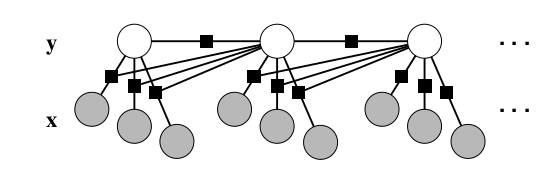
\includegraphics[width=0.7\textwidth]{Bilder/crf-modell-charles-andrew}
\caption{CRF-Modell (die Abbildung ist der Arbeit von Charles Sutton \cite{Charles/Andrew:10} entnommen)}
\label{fig:CRF-Modell}
\end{figure}

\paragraph{}
Die Formel, die die Verteilung $p(y|x)$ beschreibt, lautet 
$$
p(y|x) = \frac{1}{Z(x)}\prod_{t=1}^T\exp \lbrace \sum_{k=1}^K \theta_k f_k(y_t,y_t-1,x_t) \rbrace
$$  

Funktion $f_k$ beschreibt dabei Features, und Vektor $\theta$ - Parameter. Die Funktion $Z(x)$ ist eine Normalisierungsfunktiuon, und wird wie folgt definiert:
$$
Z(x) = \sum_y \prod_{t=1}^T\exp \lbrace \sum_{k=1}^K \theta_k f_k(y_t,y_t-1,x_t) \rbrace
$$
Vektor $x_t$ beinhaltet dabei alle Features, die benötigt werden, um Abhängigkeiten zu berechnen. 

\paragraph{}
Aber wie definiert man Features? Jenny Finkel\cite{Jenny/etal:07} hat folgende Eigenschaften definiert:
\begin{enumerate}
\item Nachbarnwörter: vorheriges Wort, nächstes Wort, alle Wörter innerhalb eines Fensters.
\item Orthographische Eigenschaften.
\item Präfixe und Suffixe.
\item Labelsequenzen.
\end{enumerate}

\subsection{Maximum Entropy based NER}

\section{Wissendatenbanke}
\subsection{SPARQL}
